\documentclass{article}
\usepackage{tikz}
\usetikzlibrary{arrows.meta,positioning,calc,shapes.geometric}
\pagestyle{empty}
\begin{document}
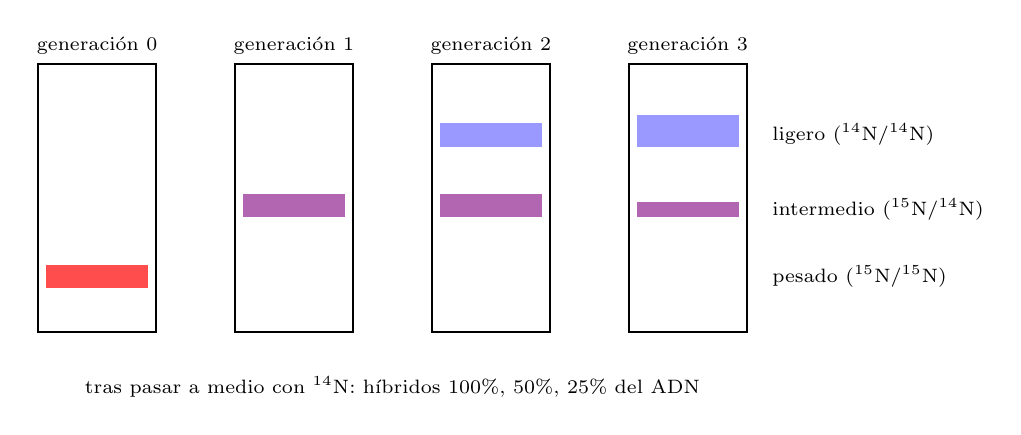
\begin{tikzpicture}

\foreach \x/\n in {0/0,2.5/1,5/2,7.5/3} {\draw[thick] (\x,0) rectangle (\x+1.5,3.4);}
\node[font=\scriptsize, above] at (0.75,3.4) {generación 0}; \node[font=\scriptsize, above] at (3.25,3.4) {generación 1}; \node[font=\scriptsize, above] at (5.75,3.4) {generación 2}; \node[font=\scriptsize, above] at (8.25,3.4) {generación 3};
\fill[red!70] (0.1,0.55) rectangle (1.4,0.85);
\fill[violet!60] (2.6,1.45) rectangle (3.9,1.75);
\fill[violet!60] (5.1,1.45) rectangle (6.4,1.75); \fill[blue!40] (5.1,2.35) rectangle (6.4,2.65);
\fill[violet!60] (7.6,1.45) rectangle (8.9,1.65); \fill[blue!40] (7.6,2.35) rectangle (8.9,2.75);
\node[font=\scriptsize, right] at (9.2,0.7) {pesado ($^{15}$N/$^{15}$N)}; \node[font=\scriptsize, right] at (9.2,1.55) {intermedio ($^{15}$N/$^{14}$N)}; \node[font=\scriptsize, right] at (9.2,2.5) {ligero ($^{14}$N/$^{14}$N)};
\node[font=\scriptsize, align=center] at (4.5,-0.7) {tras pasar a medio con $^{14}$N: híbridos 100\%, 50\%, 25\% del ADN};

\end{tikzpicture}
\end{document}
